\documentclass[12pt,a4paper]{article}
\usepackage[utf8]{vietnam}
\usepackage[T5]{fontenc}
\usepackage{graphicx}
\usepackage{hyperref}
\usepackage{geometry}
\geometry{left=2.5cm,right=2.5cm,top=2.5cm,bottom=2.5cm}
\usepackage{titlesec}
\titleformat{\section}{\bfseries\Large}{\thesection.}{1em}{}
\titleformat{\subsection}{\bfseries}{\thesubsection.}{1em}{}
\usepackage{fancyhdr}
\pagestyle{fancy}
\fancyhf{}
\rhead{Lê Thiên Quân – 24520027}
\lhead{Báo cáo đồ án môn học}
\rfoot{Trang \thepage}

\begin{document}
	
	\begin{center}
		\Large\textbf{BÁO CÁO ĐỒ ÁN MÔN HỌC} \\
		\vspace{0.5em}
		\normalsize Lớp: IT003.CTTN.P21 \\
		\vspace{2em}
		\textbf{Thông tin sinh viên} \\
	\end{center}
	
	\begin{itemize}
		\item Mã số sinh viên: \textbf{24520027}
		\item Họ và tên: \textbf{Lê Thiên Quân}
		\item Tên đề tài: \textbf{ICPC Assistant – Ứng dụng hỗ trợ thống kê và huấn luyện đội tuyển ICPC}
	\end{itemize}
	
	\vspace{1em}
	
	\section{Giới thiệu đề tài}
	
	Đồ án xây dựng một ứng dụng web hỗ trợ đội tuyển ICPC trong việc quản lý, thống kê và phân tích dữ liệu luyện tập. Hệ thống sử dụng FastAPI (Python) làm backend và HTML, CSS, JavaScript cho phần frontend. Dữ liệu được thu thập tự động từ Codeforces thông qua API chính thức.
	
	\section{Quá trình thực hiện}
	
	\subsection*{Tuần 1}
	\begin{itemize}
		\item Tìm hiểu kiến trúc FastAPI.
		\item Học cách tích hợp FastAPI với HTML/CSS/JS.
	\end{itemize}
	
	\subsection*{Tuần 2}
	\begin{itemize}
		\item Thiết kế giao diện cơ bản.
		\item Viết các hàm truy vấn API từ Codeforces.
	\end{itemize}
	
	\subsection*{Tuần 3}
	\begin{itemize}
		\item Sử dụng SQLite để lưu trữ dữ liệu tạm.
		\item Tối ưu quá trình gọi API, tránh trùng lặp.
	\end{itemize}
	
	\subsection*{Tuần 4}
	\begin{itemize}
		\item Xây dựng chức năng thống kê: số bài đã giải, biểu đồ tiến bộ, xếp hạng.
		\item Cải thiện giao diện, bố cục dữ liệu.
	\end{itemize}
	
	\section{Kết quả đạt được}
	
	\begin{itemize}
		\item Hoàn thành hệ thống cơ bản:
		\begin{itemize}
			\item Kết nối Codeforces API.
			\item Lưu trữ dữ liệu cục bộ.
			\item Thống kê bài tập, biểu đồ xếp hạng.
		\end{itemize}
		\item Giao diện trực quan, dễ sử dụng.
		\item Hạn chế: tính năng chatbot AI hỗ trợ luyện tập vẫn chưa hoàn thiện.
	\end{itemize}
	
	\section{Tài liệu tham khảo}
	
	\begin{enumerate}
		\item FastAPI Documentation – \url{https://fastapi.tiangolo.com}
		\item Codeforces API – \url{https://codeforces.com/apiHelp}
		\item SQLite Documentation – \url{https://sqlite.org}
		\item MDN Web Docs – HTML, CSS, JS – \url{https://developer.mozilla.org}
	\end{enumerate}
	
	\section*{Phụ lục 1: Demo giao diện}
	
	% Chèn hình minh họa nếu có
	\begin{figure}[h!]
		    \centering
		   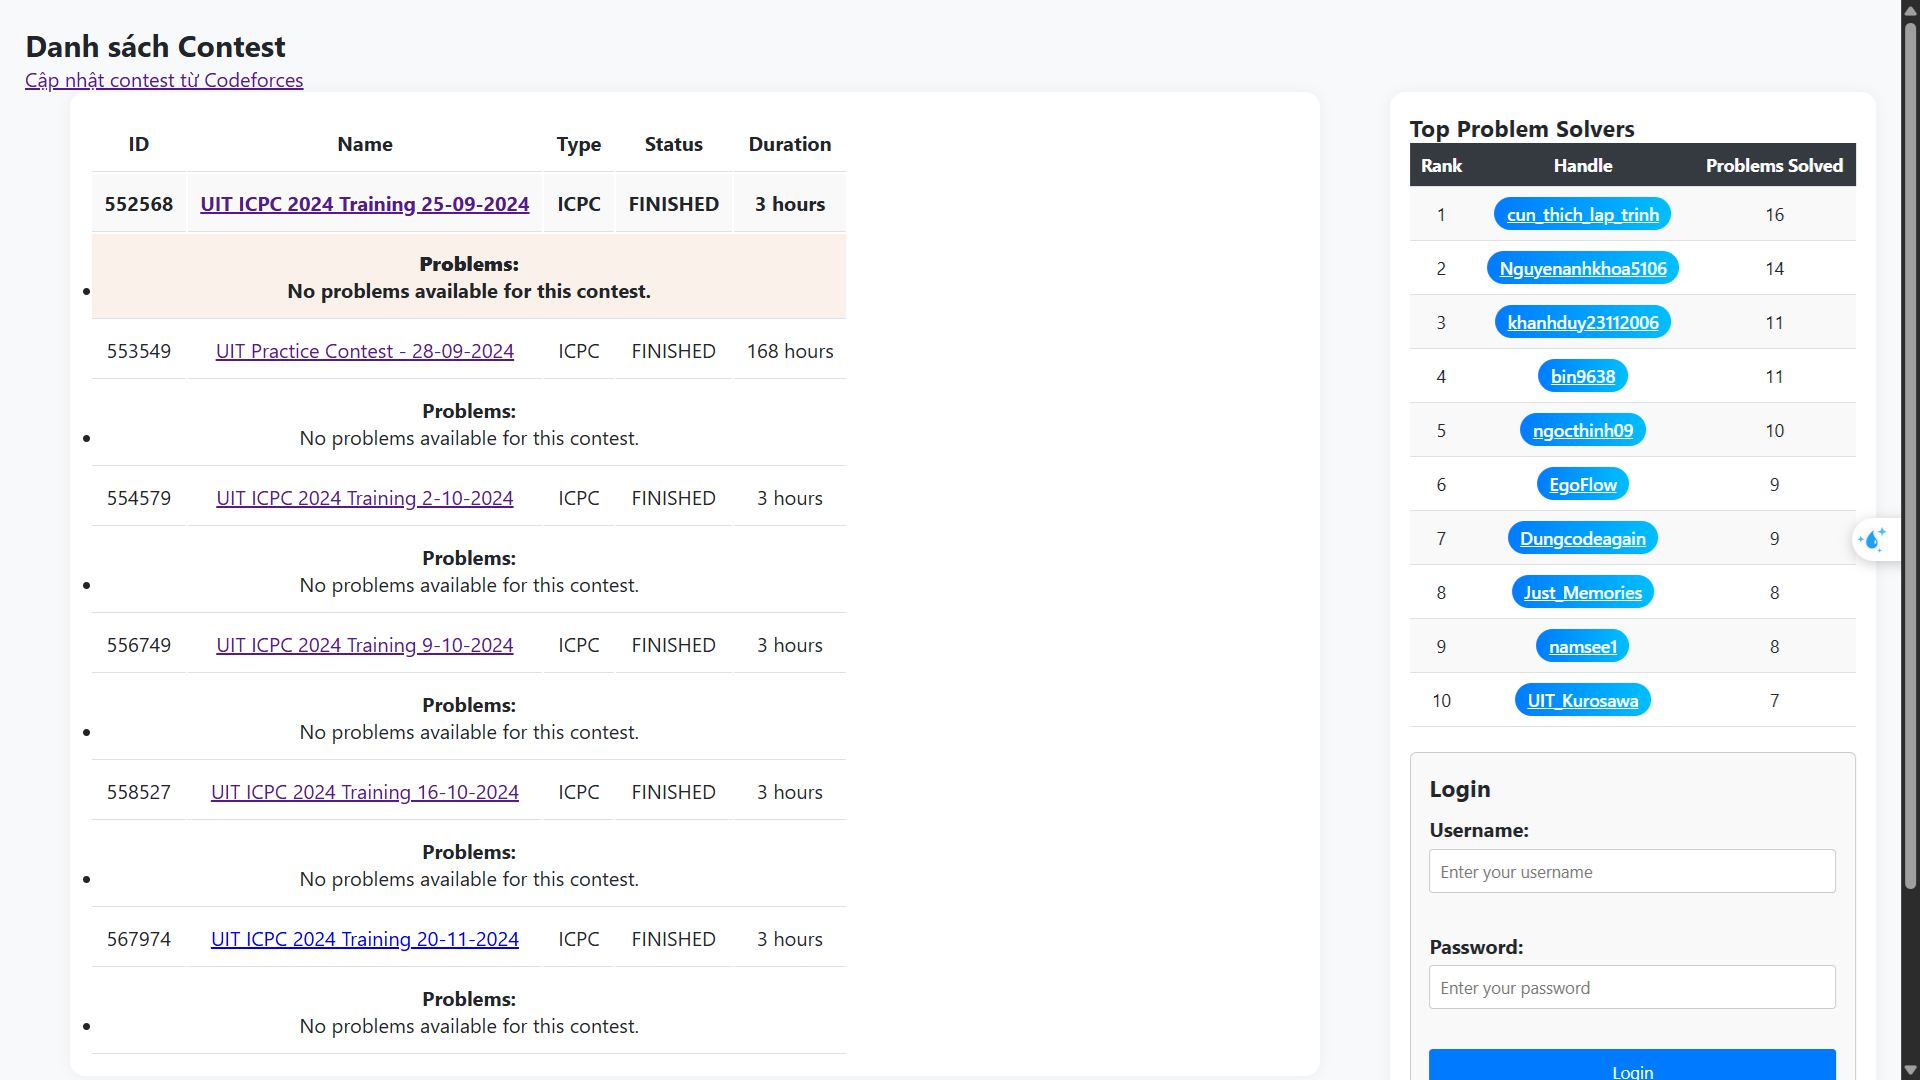
\includegraphics[width=0.8\textwidth]{test1.png}
		  \caption{Giao diện chính của trang web}
	 \end{figure}
	
	\begin{figure}[h!]
		\centering
		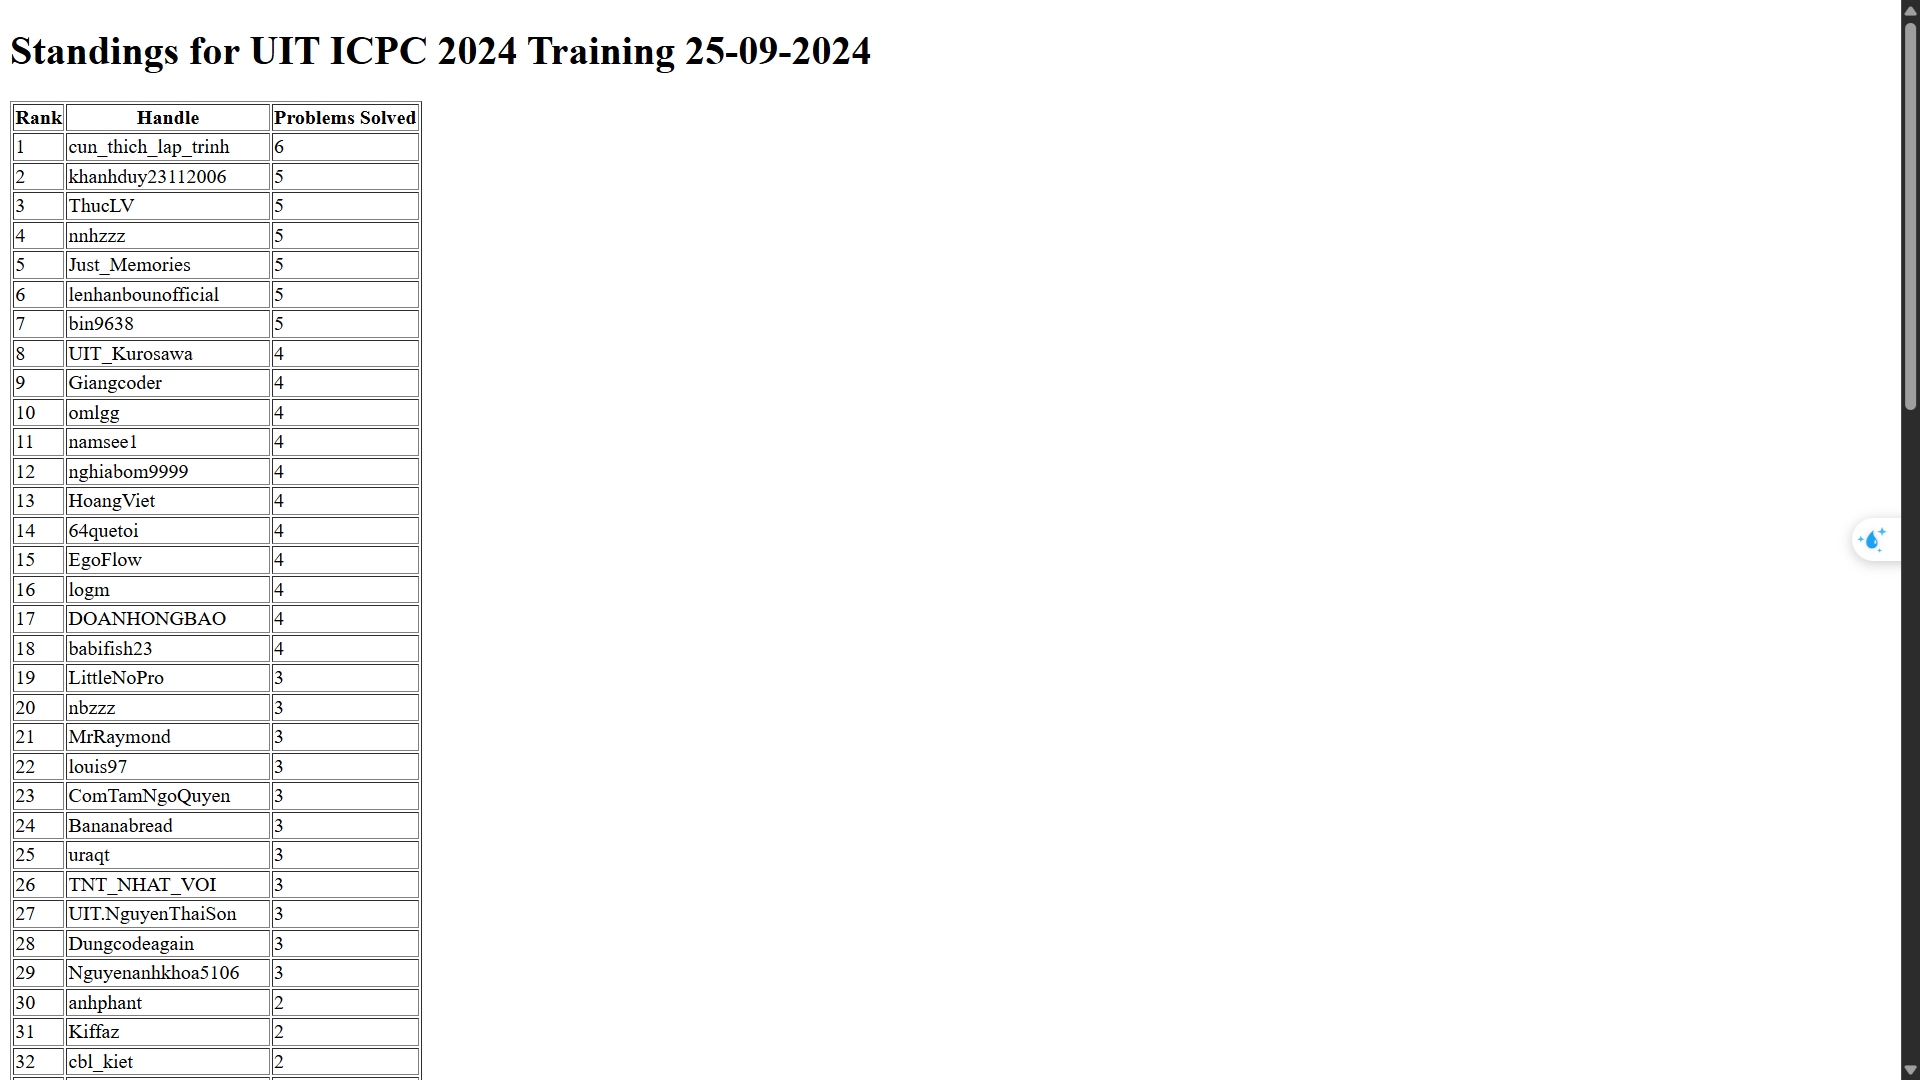
\includegraphics[width=0.8\textwidth]{test2.png}
		\caption{Giao diện của bảng xếp hạng mỗi contest}
	\end{figure}
	
	\begin{figure}[h!]
		\centering
		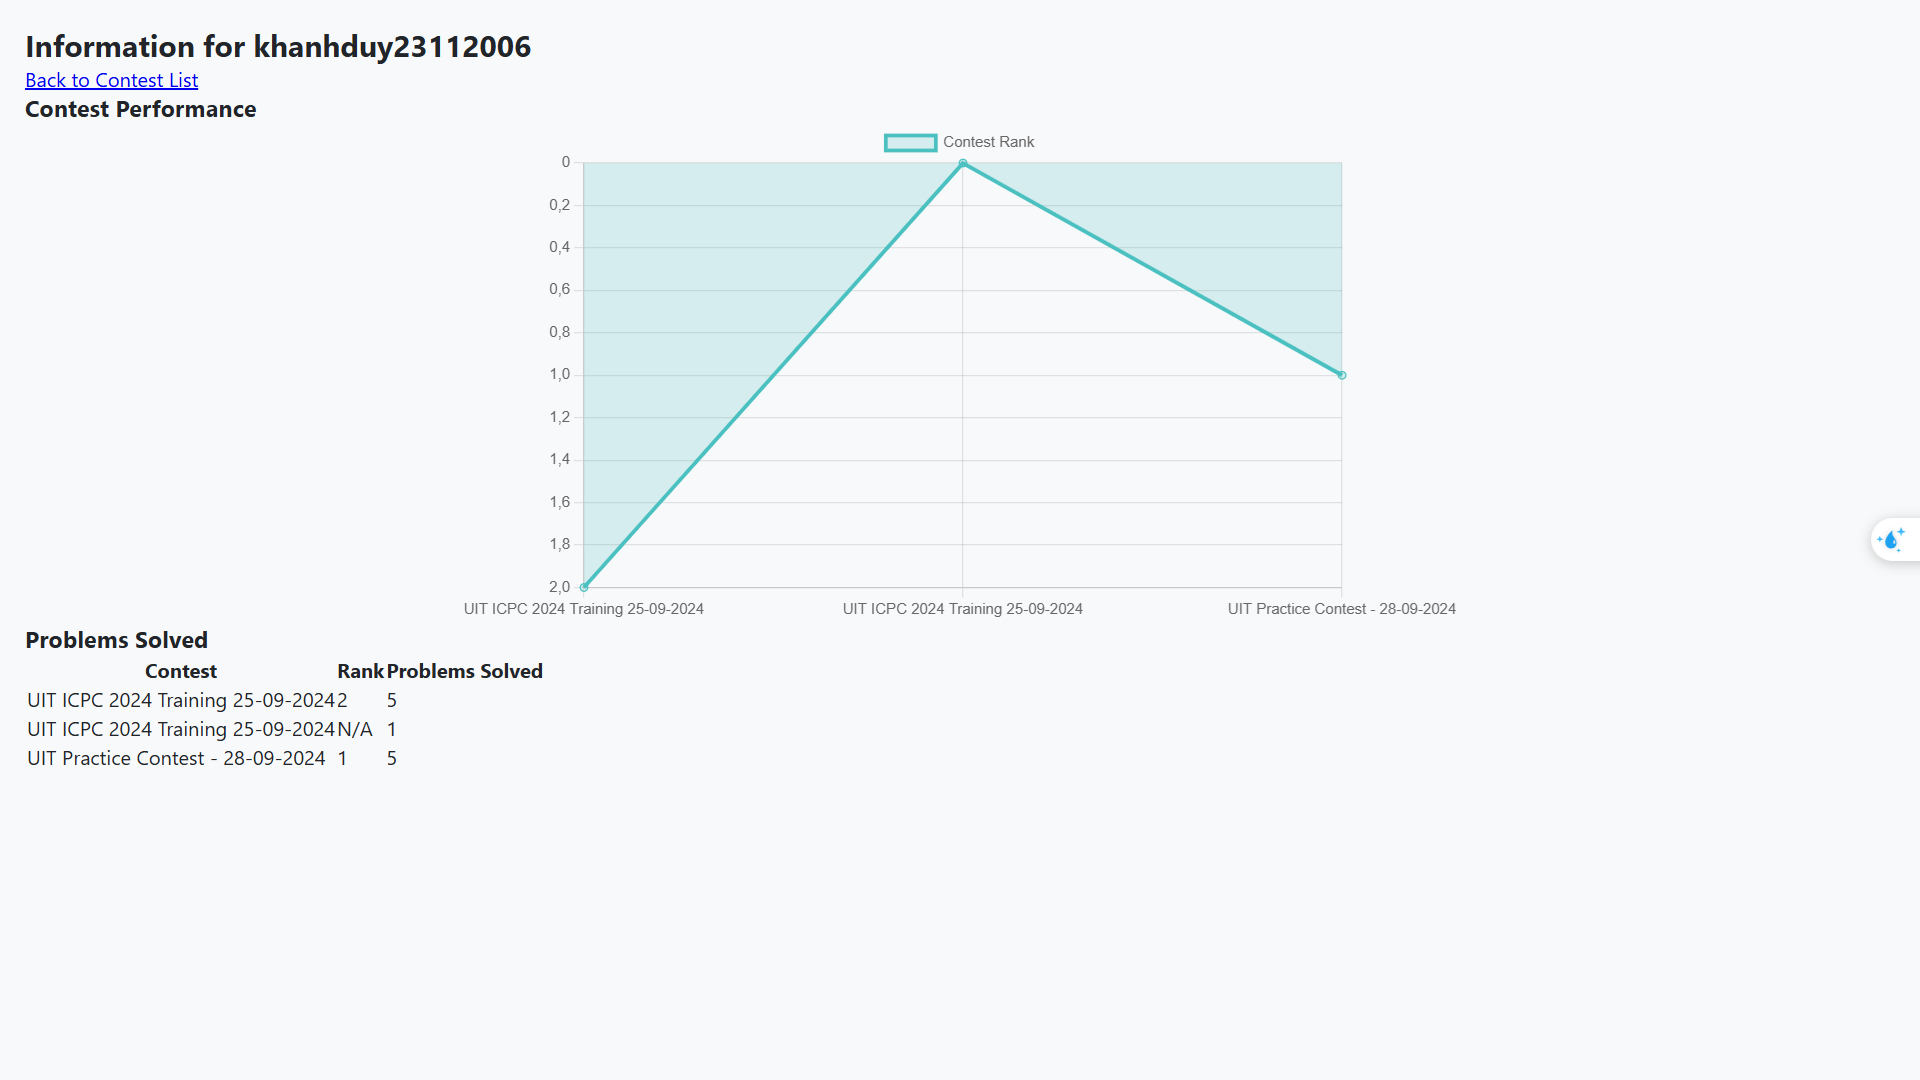
\includegraphics[width=0.8\textwidth]{test3.png}
		\caption{Biểu đồ phân tích của mỗi thành viên}
	\end{figure}
	
	\vspace{1em}
	\section*{Phụ lục 2: Trích xuất Docstring (ví dụ)}
	
	\begin{verbatim}
	File: .\login.py
	Loại: function
	Tên: authenticate_user
	Docstring:
	Authenticate a user by username and password.
	
	Args:
	username (str): The username to authenticate.
	password (str): The plain text password to verify.
	
	Returns:
	dict or None: The user dictionary if authentication is successful, otherwise None.
	============================================================
	File: .\login.py
	Loại: function
	Tên: create_access_token
	Docstring:
	Create a JWT access token.
	
	Args:
	data (dict): The data to encode in the token (e.g., user info).
	expires_delta (timedelta, optional): The time until the token expires. Defaults to 15 minutes.
	
	Returns:
	str: The encoded JWT token as a string.
	============================================================
	File: .\login.py
	Loại: function
	Tên: login_page
	Docstring:
	Render the login page.
	
	Args:
	request (Request): The incoming HTTP request.
	
	Returns:
	TemplateResponse: The rendered login.html template.
	============================================================
	File: .\login.py
	Loại: function
	Tên: login
	Docstring:
	Authenticate user and return an access token.
	
	Args:
	form_data (OAuth2PasswordRequestForm): The form data containing username and password.
	
	Raises:
	HTTPException: If authentication fails.
	
	Returns:
	dict: A dictionary containing the access token and token type.
	============================================================
	File: .\login.py
	Loại: function
	Tên: get_current_user
	Docstring:
	Retrieve the current user from the JWT token.
	
	Args:
	token (str): The JWT token from the Authorization header.
	
	Raises:
	HTTPException: If the token is invalid or missing required fields.
	
	Returns:
	dict: A dictionary containing the username and role of the user.
	============================================================
	File: .\login.py
	Loại: function
	Tên: admin_required
	Docstring:
	Dependency to ensure the current user is an admin.
	
	Args:
	current_user (dict): The current user dictionary, injected by Depends(get_current_user).
	
	Raises:
	HTTPException: If the user is not an admin.
	
	Returns:
	dict: The current user dictionary if the user is an admin.
	============================================================
	File: .\main.py
	Loại: function
	Tên: fetch_contest_info
	Docstring:
	Fetch contest information from the Codeforces API for a given contest ID.
	
	Args:
	contest_id (int): The ID of the contest to fetch.
	
	Returns:
	dict or None: The contest information dictionary if successful, otherwise None.
	============================================================
	File: .\main.py
	Loại: function
	Tên: update_contests
	Docstring:
	Update contests and standings in the database from the Codeforces API.
	
	Returns:
	dict: A message indicating how many contests were added or updated.
	============================================================
	File: .\main.py
	Loại: function
	Tên: update_contests_get
	Docstring:
	HTTP GET endpoint to trigger updating contests and standings.
	
	Returns:
	dict: A message indicating how many contests were added or updated.
	============================================================
	File: .\main.py
	Loại: function
	Tên: contest_standings
	Docstring:
	Render the standings page for a specific contest.
	
	Args:
	request (Request): The incoming HTTP request.
	contest_id (int): The ID of the contest.
	
	Returns:
	TemplateResponse: The rendered standings.html template.
	============================================================
	File: .\main.py
	Loại: function
	Tên: fetch_contest_standings
	Docstring:
	Fetch standings for a given contest from the database.
	
	Args:
	contest_id (int): The ID of the contest.
	
	Returns:
	list: A list of dictionaries containing handle, rank, and problems solved.
	============================================================
	File: .\main.py
	Loại: function
	Tên: member_info
	Docstring:
	Render the statistics page for a specific member (user).
	
	Args:
	request (Request): The incoming HTTP request.
	handle (str, optional): The handle (username) of the member.
	
	Returns:
	TemplateResponse: The rendered member.html template with member statistics.
	============================================================
	File: .\main.py
	Loại: function
	Tên: fetch_problem_names
	Docstring:
	Fetch all problem names for a given contest from the database.
	
	Args:
	contest_id (int): The ID of the contest.
	
	Returns:
	list: A list of problem names for the contest.
	============================================================
	File: .\main.py
	Loại: function
	Tên: home
	Docstring:
	Render the home page with contest list, top solvers, and problems for each contest.
	
	Args:
	request (Request): The incoming HTTP request.
	
	Returns:
	TemplateResponse: The rendered home.html template.
	============================================================
	File: .\backend\models.py
	Loại: class
	Tên: Contest
	Docstring:
	ORM model for a programming contest.
	
	Attributes:
	id (int): Primary key, unique contest ID.
	name (str): Name of the contest.
	type (str): Type of the contest (e.g., ICPC, CF).
	phase (str): Current phase of the contest.
	durationSeconds (int): Duration of the contest in seconds.
	standings (list[Standing]): List of standings for this contest.
	problems (list[Problem]): List of problems for this contest.
	============================================================
	File: .\backend\models.py
	Loại: class
	Tên: Solver
	Docstring:
	ORM model for a solver (participant).
	
	Attributes:
	id (int): Primary key, unique solver ID.
	handle (str): Unique handle/username of the solver.
	solved_count (int): Total number of problems solved by the solver.
	============================================================
	File: .\backend\models.py
	Loại: class
	Tên: Problem
	Docstring:
	ORM model for a problem in a contest.
	
	Attributes:
	id (int): Primary key, unique problem ID.
	name (str): Name of the problem.
	topics (str): Topics/tags associated with the problem.
	contest_id (int): Foreign key to the contest this problem belongs to.
	contest (Contest): Relationship to the Contest model.
	============================================================
	File: .\backend\models.py
	Loại: class
	Tên: Standing
	Docstring:
	ORM model for a contest standing (result for a solver in a contest).
	
	Attributes:
	id (int): Primary key, unique standing ID.
	handle (str): Handle/username of the solver.
	rank (int): Rank achieved by the solver in the contest.
	problems_solved (int): Number of problems solved by the solver in the contest.
	contest_id (int): Foreign key to the contest.
	contest (Contest): Relationship to the Contest model.
	============================================================
	File: .\backend\sign_url.py
	Loại: function
	Tên: generate_random_string
	Docstring:
	Generate a random string of fixed length.
	
	Args:
	length (int, optional): The length of the random string. Defaults to 6.
	
	Returns:
	str: A random alphanumeric string of the specified length.
	============================================================
	File: .\backend\sign_url.py
	Loại: function
	Tên: build_signed_url
	Docstring:
	Generate a signed URL for the Codeforces API.
	
	Args:
	method_name (str): The API method name (e.g., 'contest.standings').
	params (dict): The parameters to include in the API request.
	
	Returns:
	str: The signed URL ready for use with the Codeforces API.
	\end{verbatim}
	
	\section*{Link github của dự án:}
	
	\href{https://github.com/lethienquan28052006/icpcmanagementwebapp}{Link ở đây}
	
\end{document}
